\section{Infrastructure de traitement des flux de données}\label{sec:rw:sgfd:infra}
L'architecture des systèmes de gestions de flux de données diffère. Toutefois, plusieurs concepts fondateurs sont communément utilisés pour l'évaluation des requêtes. Tout d'abord, nous présentons les principes des infrastructures des SGFD. Ceux-ci sont fondamentaux pour permettre l'intégration de systèmes hétérogènes. Ensuite, nous détaillons les principes architecturaux développés particulièrement pour permettre aux infrastructures de supporter les grandes quantités de données.

\subsection{Éléments d'architecture de l'évaluation de requête}
Le modèle théorique permet de formaliser la sémantique exacte des expressions de requêtes. L'évaluation de ces requêtes soulève des difficultés, notamment en ce qui concerne la gestion de la mémoire.

\subsubsection{Les résultats intermédiaires}
Comme présenté précédemment en section~\ref{sec:rw:supervision:datastream}, la gestion de flux de données se décompose en trois composants principaux : les sources, les opérateurs et les puits. Les opérateurs consomment une ou plusieurs entités (un flux par exemple) et produisent une nouvelle entité. Ces entités sont des composants représentant les résultats intermédiaires comme présenté par A, B, X et Y dans la figure~\ref{fig:rw:sgfd:implem}.
\begin{figure}[ht]
    \centering
    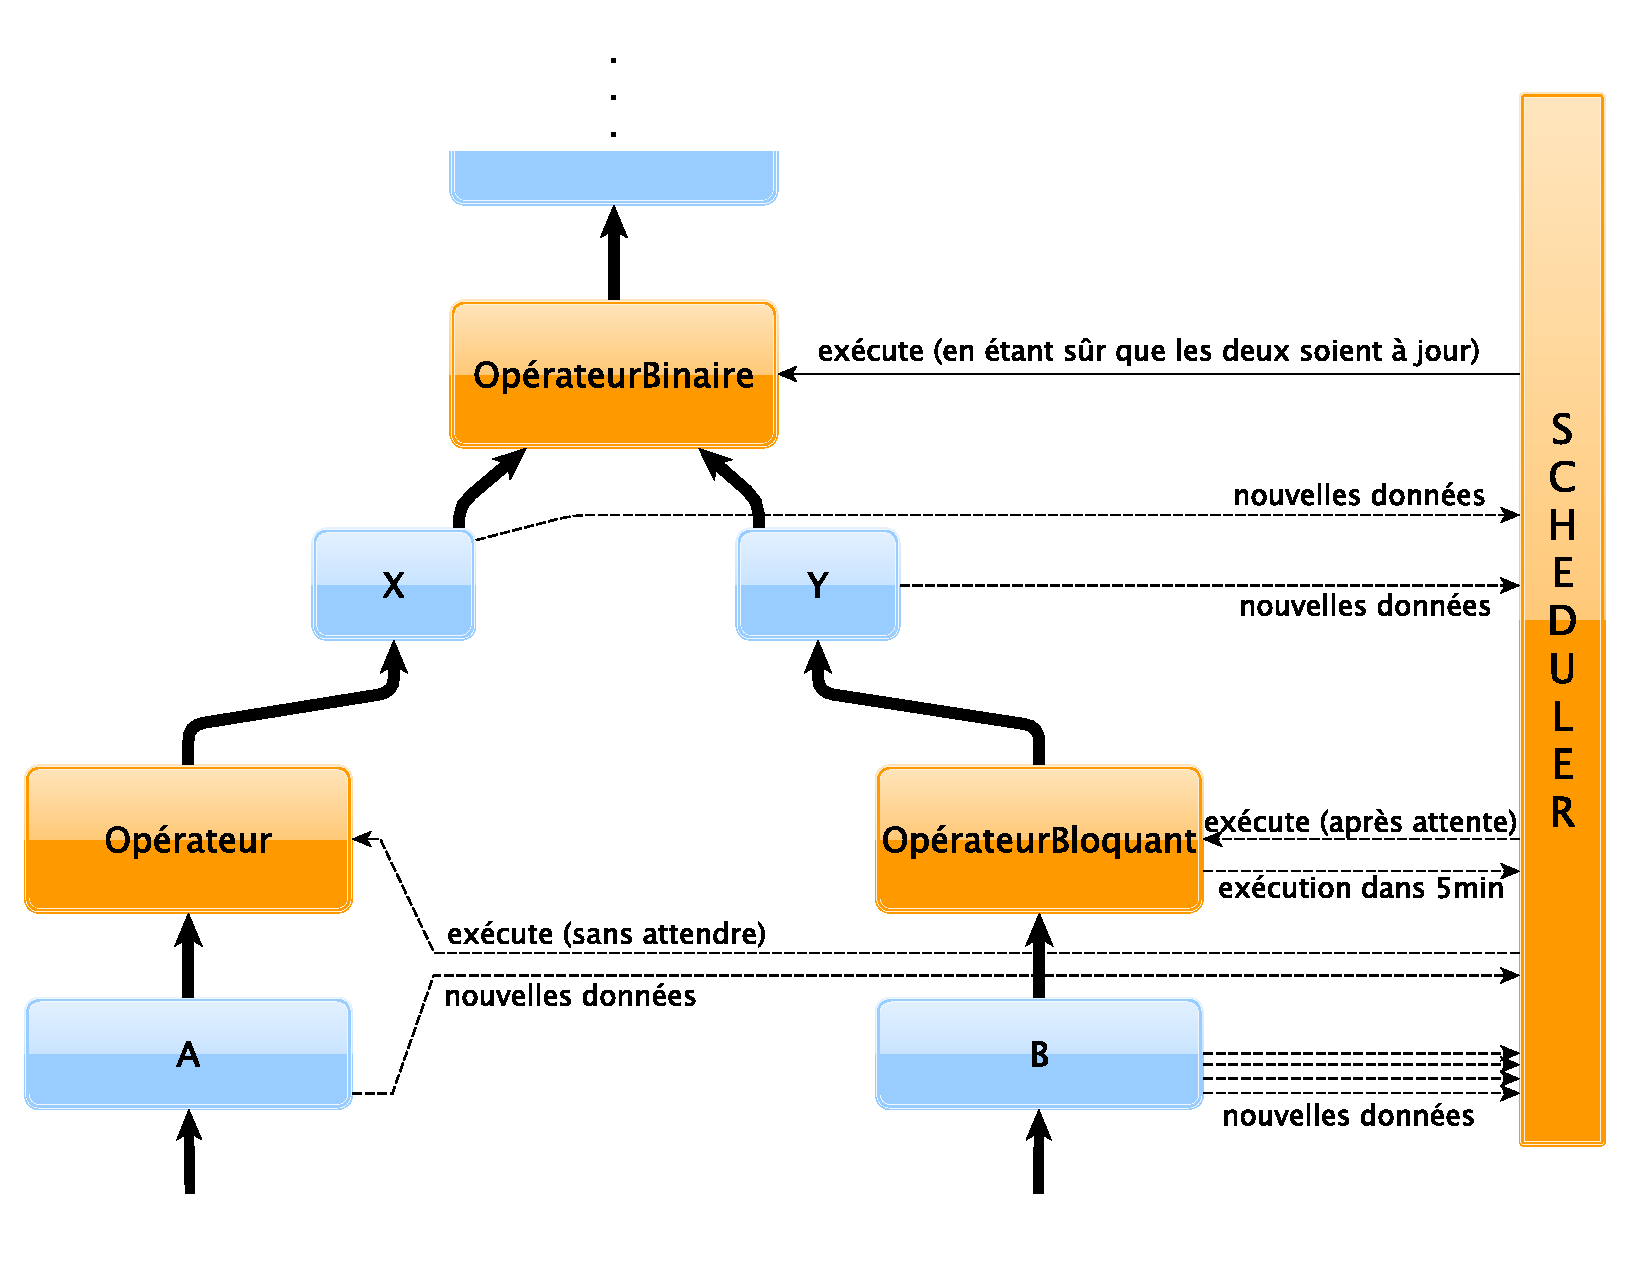
\includegraphics[width=0.8\textwidth]{rw-sgfd-implem}
    \caption{Structure de l'évaluation d'une requête continue}\label{fig:rw:sgfd:implem}
\end{figure}

Ces composants utilisent des mémoires tampons et occasionnellement des supports persistants~\cite{Abadi:aurora}. Ces composants sont manipulés par une interface d'appel très simple en général basé sur les primitives \textit{push} et \textit{pop} telle une pile. Or, lors de l'évaluation de la requête, il est nécessaire de vider le plus rapidement possible ces mémoires pour éviter les saturations. Certains travaux introduisent des opérations plus complexes dans ces composants tels que des primitives d'ordres ou de sélection comme dans les \textit{SweepArea} de \textit{PIPES}~\cite{Kramer:semantics}. Toutefois, il n'est pas toujours possible de consommer directement ces mémoires tampons.

\subsubsection{L'exécution}
Deux types d'exécutions sont référencés : les non-bloquantes et les bloquantes~\cite{Babcock:issues}. Originellement, un opérateur \textit{bloquant} est \enquote{\it un opérateur qui n'est pas capable de produire son premier n-uplet tant que l'ensemble de son entrée n'a pas été consommé}. Les opérateurs souvent cités sont les agrégats. Par la suite, grâce aux recherches sur les fenêtres~\cite{Maier:semantics}, le terme est généralisé aux opérations de fenêtrages dont le décalage est différent de \textit{1 n-uplet}.

Ainsi, les opérateurs bloquants ne sont pas seulement cadencés par les données de son entrée. Ils ont leur propre cycle de vie, ce qui les rend plus compliqués à exécuter. Le module d'ordonnancement (\textit{scheduler})~\cite{Carney:scheduling} est présent dans la plupart des implémentations supportant ce type d'opérateur. Ce composant a pour tâche de décider quel opérateur exécuter et quand.

Dans la figure~\ref{fig:rw:sgfd:implem}, le \textit{scheduler} contrôle l'exécution des trois opérateurs. Le premier \textit{Opérateur} est un opérateur non-bloquant, ainsi lors de l'arrivée d'une nouvelle donnée dans \textit{A}, il acquiert le droit de s'exécuter. L'\textit{OpérateurBloquant} quant à lui décide de lui même qu'il veuille s'exécuter 5 minutes plus tard (pour une fenêtre par exemple). Ainsi, \textit{B} accumule des données et envoie d'un bloc l'ensemble de ses données au moment où l'opérateur décide de finalement les consulter. L'\textit{OpérateurBinaire} est non-bloquant, néanmoins, le \textit{scheduler} doit bien vérifier que \textit{X} et \textit{Y} sont à jour avant de lancer l'exécution. Il est en effet possible que \textit{X} soit à jour mais qu'un traitement soit encore en attente pour \textit{Y}.

Quant à la communication entre les composants résultats et les opérateurs, les mécanismes de souscriptions (\textit{publish/subscribe} ou \textit{push})~\cite{Eugster:publishsubscribe} ne sont pas toujours adoptés. En effet, au lieu d'appliquer strictement l'approche événementielle, l'infrastructure peut nécessiter de privilégier une approche par appel (\textit{pull}).

Par exemple, le moteur MXQuery~\cite{Botan:MXQuery} est un SGFD dont la particularité est de traiter des documents \textit{XML} tels que \textit{RSS} (flux d'actualités). Ce moteur ne supporte que l'approche \textit{pull} en entrée. A la différence, un SGFD plus généraliste tel que STREAM doit supporter un mécanisme événementiel. La gestion de l'hétérogénéité de l'évolution des données s'applique ainsi au niveau de l'infrastructure d'évaluation des requêtes.

\subsection{Passage à l'échelle}
Les travaux sur l'architecture des SGFD se sont beaucoup concentré sur son passage à l'échelle en terme de volume de données. Le volume de données se décline en deux dimensions dans le cadre des flux de données : le débit d'un flux et le nombre de flux sources. Nous analysons dans un premier temps le \textit{load-shedding} prévu pour gérer des débits trop importants pour le SGFD. Puis, nous détaillons le procédé de \textit{désignation} permettant de maîtriser le nombre de flux sources. Enfin, nous présentons les choix d'architectures distribués pratiqués pour subvenir aux grands volumes de données en général.

\subsubsection{Load-shedding}
Contrairement aux approches classiques de gestion de base de données, il est important de voir que dans la gestion de flux certaines optimisations dégradent la qualité des résultats. L'objectif du \textit{shedding} est de fournir les résultats les plus pertinents possibles avec des contraintes d'espace mémoire, de temps de réponse ainsi que de charge réseau. En effet, comme la gestion de flux fonctionne de manière continue, une congestion dans le processus de traitement implique des retards et des complications pouvant aller jusqu'à une saturation du moteur.

L'idée du \textit{load-shedding} est de pouvoir abaisser ou limiter le taux de n-uplet pour pouvoir les traiter sans introduire de retard. Dans les travaux fondateurs~\cite{Tatbul:window,Tatbul:load-shedding}, l'idée est de pouvoir surveiller le traitement des requêtes afin de reconnaitre les points d'engorgements et d'y implanter des opérateurs de \textit{shedding}. Afin de garantir un certain taux de réussite, la politique utilisée est dirigée par des indications de qualité de services déterminant quelles données sont utiles. En effet, en prenant en entrée un graphe représentant \textit{valeur} $\mapsto$  \textit{taux de suppression acceptable}. Par exemple, dans le cadre d'une surveillance d'incendie, le taux de \textit{shedding} pour les températures inférieure à 20ºC pourrait être très fort. Le critère de sélection afin d'autoriser la suppression d'une données peut se faire de façons différentes :
\begin{itemize}
 \item Par un histogramme et un choix sur le nombre de tuple résultant~\cite{Han:join}
 \item Par un calcul probabiliste pour privilégier un flux plutôt qu'un autre pour sa productivité~\cite{Han:join}
 \item Par des raisonnements sur l'age des n-uplets~\cite{Srivastava:join}
\end{itemize}

\subsubsection{Désignation}\label{sec:rw:sgfd:infra:designation}
Plus le nombre de sources de données augmente, plus il devient difficile de maîtriser lesquelles sont concernées par la requête que l'utilisateur souhaite déployer. Une requête par désignation est une requête utilisant une autre requête pour désigner les sources de données à lire. Par exemple : \enquote{\it Le flux des mesures des capteurs de température du batiment A}. Dans cette requête, il est nécessaire de d'abord faire une interrogation sur l'expression \enquote{\it Quels sont les capteurs situés dans le batiment \textit{A} et de type \textit{température}} avant de déployer la requête.

Ce procédé est implanté dans notamment SStreamWare, HiFi et GSN~\cite{Aberer:gsn}. Le passage à l'échelle en nombre de sources de données est particulièrement notable dans \textit{GSN} qui vise un internet de capteurs. Son architecture est naturellement pair-à-pair. L’interrogation continue sur ce système peut se faire par le déploiement de nouveaux capteurs virtuels. La désignation est centrale car la formation d’un capteur virtuel à partir d’autres sources est possible. Toutefois, du fait de l’absence de méta-données la puissance d'expression de cette requête de désignation est limitée. Dans SStreamWare et HiFi, au contraire, le support des méta-données telles que leur position, leur type ou leur fréquence d'émission facilite la sélection des sources concernés.

\subsubsection{Architecture distribué}
La distribution des SGFD pour mieux supporter les volumes de données fait parti des techniques classiques. La structure même des requêtes en forme d'arbre d'opérateurs permet la mise en œuvre naturelle de structures hiérarchiques. En effet, des systèmes tels que \textit{Borealis}~\cite{Abadi:borealis} (historiquement, l'évolution d'\textit{Aurora}) permettent de distribuer le calcul d'une requête sur plusieurs nœuds.

La distribution d'un calcul emmène des problèmes de synchronisation, de répartition de charge, des tolérances aux fautes et de latence de traitement. Des recherches~\cite{Hwang:distributed, Tucker:heartbeat} ont été faites sur ces points pour permettre une évaluation des requêtes exacte avec une latence faible.

L'approche hiérarchique permet de faire du traitement à plusieurs niveaux. Ces niveaux peuvent avoir un rôle bien défini dans le traitement des données. C'est le cas pour \textit{HiFi}~\cite{Franklin:hifi} présentant cinq niveaux de traitement des données. À chaque niveau correspond un type d'opération et à une localisation bien défini :
\begin{itemize}
	\item[\textbf{Nettoyage} :] Application de filtres sur les données pour enlever les anomalies. Traitement situé sur le capteur.
	\item[\textbf{Lissage} :] Interpolation des mesures perdues. Utilisation d'agrégats sur les fenêtres. Traitement situé sur la station d'accueil des capteurs.
	\item[\textbf{Arbitrage} :] Consolidation des données. Suppression de données dupliquées, agrégations des données nécessaires au niveau suivant. Traitement situé au niveau d'un batiment.
	\item[\textbf{Validation} :] Applications de règles métiers pour valider les données. Utilisation principale de jointures. Traitement situé à un niveau régional.
	\item[\textbf{Analyse} :] Support de décisions tels que vu dans la section~\ref{sec:rw:supervision:warehouse}. Traitement situé au centre de commandement.
\end{itemize}

Cette approche a été généralisé dans \textit{SStreamWare}~\cite{Gurgen:sstreamware} avec les \textit{sites de contrôle} (plus haut niveau hiérarchique) et les \textit{passerelles}. Ces dernières sont capables d'accueillir des capteurs (virtuels ou non), ainsi que d'exécuter une requête de flux sur les capteurs accueillis ou sur des flux externes venant d'une autre passerelle. Le site de contrôle est distribue l'exécute des requêtes sur les différentes passerelles.

\subsection{Intégration de systèmes de gestion de flux de données}
Les implémentations de SGFD diffèrent en terme d'architecture, de modèle de données, de langage de requête et même de paradigme d'exécution. En ce sens, le système Exoengine~\cite{Duller:virtualdsms} virtualise les éléments qui composent un SGFD quelconque. L'implémentation de celui-ci se fait avec une approche orienté service. Ainsi, les divers composants représentant les résultats intermédiaires exposent deux interfaces de services, l'entrée et la sortie. Ces composants sont appelés \textit{canaux}. Il devient désormais possible de relier naturellement les composants entre eux afin de gérer le flot des données formés par les \textit{canaux} pour les unir, les chaîner ou les disperser. Ainsi, tout traitement est virtualisé par un \textit{slet} qui possède un ou plusieurs ports en entrée pouvant se connecter à des \textit{canaux} et fournit un port de sortie qui est connecté à un autre \textit{canal}.

\begin{figure}[ht]
    \centering
    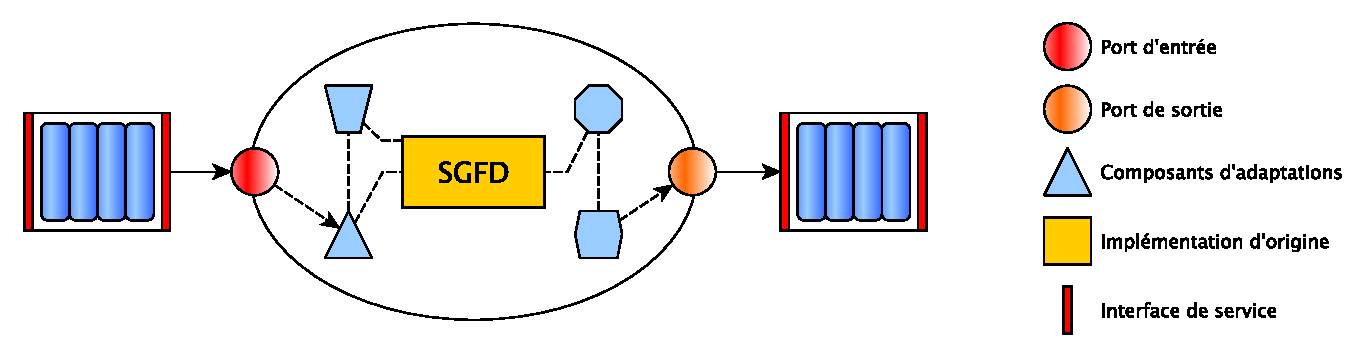
\includegraphics[width=0.8\textwidth]{rw-sgfd-virtualslet}
    \caption{Un \textit{slet} virtuel permettant d'abstraire le fonctionnement d'un SGFD}\label{fig:rw:sgfd:virtualslet}
\end{figure}
La figure~\ref{fig:rw:sgfd:virtualslet} montre un tel \textit{slet} virtuel. L'intérêt d'une telle approche est non seulement de pouvoir gérer l'hétérogénéité des SGFD mais aussi de :
\begin{itemize}
	\item Rendre un système distribuable. En implémentant des canaux réseaux dont l'entrée est sur une machine et la sortie sur une autre, il devient possible d'avoir une communication entre deux systèmes distribués. L'utilisation du même système sur plusieurs nœuds réseaux permet la distribution du calcul bien que le SGFD originel ne le supporte pas.
	\item Convertir un système \textit{pull} en système \textit{push} et inversement. L'hétérogénéité des mécanismes de récupération des données est gérée grâce à l'abstraction de service car les interfaces de services des canaux supportent les deux modes de fonctionnements.
	\item Utilisation de plusieurs modèles de données. Les canaux transmettent des objets. Les objets peuvent être la représentation de données relationnelles ou semi-structurées. Des \textit{slets} de conversions permettent de faire fonctionner deux moteurs avec des données hétérogènes.
	\item Remplacement d'un composant à chaud. L'utilisation de l'approche à service permet aussi une bonne gestion du cycle de vie des composants. Ainsi, l'administration des requêtes et des composants (\textit{slets} ou \textit{canaux}) peut se faire pendant que le système est en fonctionnement.
\end{itemize}

Toutefois, l'intégration d'SGFD n'est valable que d'un point de vue infrastructure. En effet, la mise en œuvre entre les différents systèmes suppose que l'utilisateur est capable de traduire la sémantique de sa requête dans le langage utilisé par chaque système. Or, nous avons vu qu'il n'existe pas de langage universel permettant de traduire la sémantique de chacun.
